\chapter{Introducción}

La dificultad para mantener la coherencia en sistemas cuánticos ha sido siempre un gran obstáculo en el desarrollo de
la computación cuántica. Por este motivo, la corrección cuántica de errores ha sido siempre un campo de gran interés
en el ámbito del procesamiento de información cuántica \citep{qecb}.

En este sentido, la publicación del código de \cite{shor95} fue un avance de gran interés ya que fue el primer
algoritmo de corrección cuántica de errores funcional y abrió la puerta para superar el obstáculo frente al que se encontraba el desarrollo de la computación cuántica. Se trata de un código degenerado que permite la corrección de un error de amplitud y un error de fase en un qubit.

No obstante, mientras que la implementación del código propiamente dicho se encuentra bien documentada en fuentes
tales como Quantum Computation and Quantum Information \citep{nielsenchuang} o el artículo original de \cite{shor95}, no se han encontrado implementaciones específicas del circuito correspondiente al cálculo del síndrome. Así pues, este trabajo pretende rellenar este vacío aportando posibles implementaciones de dicho circuito contempladas desde diferentes prismas.

\textbf{¿Me pregunto si esto iría mejor en el apartado de objetivos? Las dos opciones principales ante las que nos encontramos son: priorizar el ahorro de qubits reutilizando los mismos a costa de un mayor consumo energetico, utilizar más qubits.}

















---------------------------------------------

El primer capítulo es siempre una introducción. En ella debes resumir de forma esquemática pero suficientemente clara lo esencial de cada una de las partes del trabajo. La lectura de este primer capítulo ha de dar una primera idea clara de lo que se pretendía, las conclusiones a las que se ha llegado y del procedimiento seguido.

Como tal, es uno de los capítulos más importantes de la memoria. Las ideas principales a transmitir son la identificación del problema a tratar, la justificación de su importancia, los objetivos generales (a grandes rasgos) y un adelanto de la contribución que esperas hacer.

Típicamente una introducción tiene tres apartados: Motivación, Planteamiento del trabajo, Estructura del trabajo. (Texto Normal del menú de estilos.)

(Ejemplo de nota al pie\footnote{Ejemplo de nota al pie.}.)

\section{Motivación/justificación del tema a tratar}

¿Cuál es el problema que quieres tratar?

¿Cuáles crees que son las causas?

¿Por qué es relevante el problema?

A continuación, se indica con un ejemplo cómo deben introducirse los títulos y las fuentes en Tablas y Figuras.

\begin{table}[t]
	\begin{center}
	\caption{Ejemplo de tabla con sus principales elementos.}
	\label{tab:tab-1}
	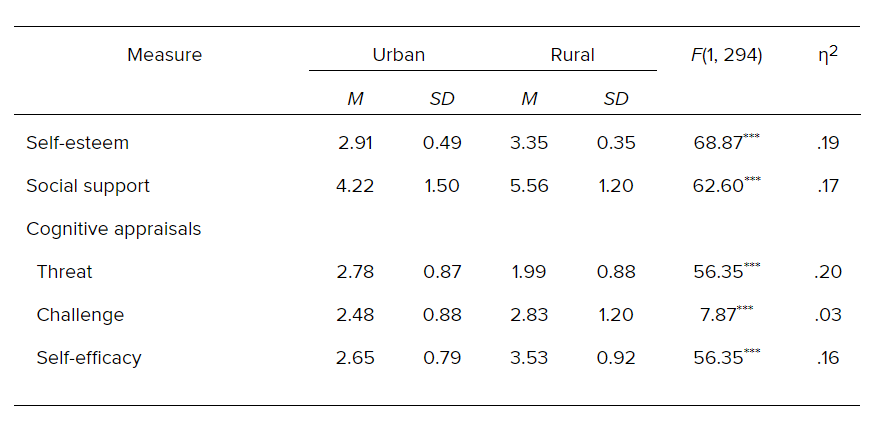
\includegraphics[width=4.90737in,height=2.42708in]{tabla}

	\small Fuente: American Psychological Association, 2020e.
	\end{center}
\end{table}

\begin{figure}[ht]
	\begin{center}
		\caption{Ejemplo de figura realizada para nuestro trabajo.}
		\label{fig:fig-1}
		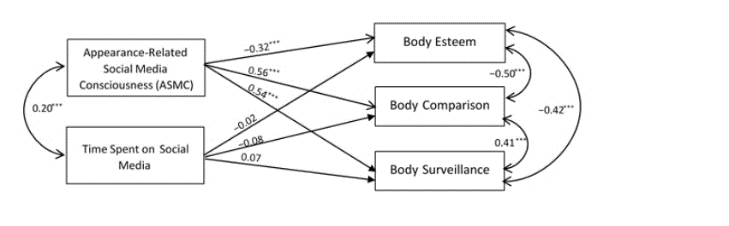
\includegraphics[width=4.90737in,height=2.42708in]{figura}

		\small Fuente: American Psychological Association, 2020f.
	\end{center}
\end{figure}

\section{Planteamiento del trabajo/problema}

¿Cómo se podría solucionar el problema?

¿Qué es lo que se propone?

Aquí describes tu objetivo en términos generales.

\section{Estructura del trabajo}

Aquí describes brevemente lo que vas a contar en cada uno de los capítulos siguientes.